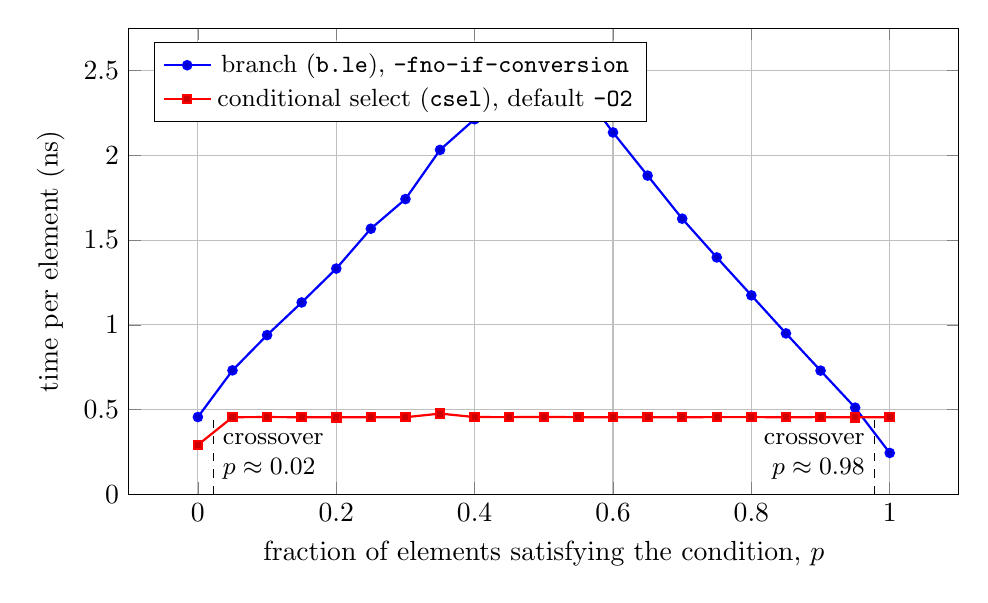
\begin{tikzpicture}
\begin{axis}[width=\textwidth, height=7.5cm, xlabel={fraction of elements satisfying the condition, $p$}, ylabel={time per element (ns)}, grid=major, ymin=0,
  legend pos=north west, legend style={font=\small}]
\addplot+[mark=*, mark size=1.5pt, thick, blue] coordinates {(0.0,0.4556) (0.05,0.731) (0.1,0.9392) (0.15,1.1318) (0.2,1.3317) (0.25,1.567) (0.3,1.742) (0.35,2.0323) (0.4,2.2132) (0.45,2.4286) (0.5,2.5002) (0.55,2.4114) (0.6,2.1352) (0.65,1.8805) (0.7,1.6262) (0.75,1.3976) (0.8,1.1737) (0.85,0.9492) (0.9,0.7295) (0.95,0.5109) (1.0,0.2436)};
\addlegendentry{branch (\texttt{b.le}), \texttt{-fno-if-conversion}}
\addplot+[mark=square*, mark size=1.5pt, thick, red] coordinates {(0.0,0.2913) (0.05,0.4548) (0.1,0.4554) (0.15,0.4547) (0.2,0.4542) (0.25,0.4546) (0.3,0.4545) (0.35,0.476) (0.4,0.4554) (0.45,0.455) (0.5,0.456) (0.55,0.4548) (0.6,0.4547) (0.65,0.4549) (0.7,0.4547) (0.75,0.4552) (0.8,0.4552) (0.85,0.4547) (0.9,0.4551) (0.95,0.4541) (1.0,0.455)};
\addlegendentry{conditional select (\texttt{csel}), default \texttt{-O2}}
\draw[dashed] (axis cs:0.022125081228057324,0) -- (axis cs:0.022125081228057324,0.448) node[pos=0.5, right, font=\small, align=left] {crossover\\$p \approx 0.02$};
\draw[dashed] (axis cs:0.9778749187719427,0) -- (axis cs:0.9778749187719427,0.448) node[pos=0.5, left, font=\small, align=right] {crossover\\$p \approx 0.98$};
\end{axis}
\end{tikzpicture}